\documentclass[11pt]{article}

\usepackage[margin=1in, headheight=14.5pt]{geometry}
\usepackage{amsfonts, amsmath, amssymb}
\usepackage[none]{hyphenat}
\usepackage{fancyhdr}
\usepackage[spanish]{babel}
\usepackage[spanish, calc]{datetime2}
\usepackage{fmtcount}
\usepackage{graphicx}
\usepackage{float}
\usepackage[nottoc, notlot, notlof]{tocbibind}
\usepackage{tocloft}
\usepackage[utf8]{inputenc}
\usepackage{parskip}
\usepackage{xcolor}
\usepackage{cancel}
\usepackage{textcomp}
\usepackage{pgfplots}
\usepackage{tikz}
\usepackage{polynom}
\usetikzlibrary{datavisualization}
\usetikzlibrary{datavisualization.formats.functions}
\pgfplotsset{compat=1.15}
\usepackage{mathrsfs}
\usetikzlibrary{arrows}

\newcommand{\dropsign}[1]{\smash{\llap{\raisebox{-.5\normalbaselineskip}{$#1$\hspace{2\arraycolsep}}}}}%


\parindent 0ex

\pgfplotsset{width=10cm,compat=1.9}

\def\imj{\mathrm{j}}
\def\sen{\mathrm{sen}}

\newcommand{\lapl}[1]{\mathscr{L} \left\lbrace {#1} \right\rbrace}
\newcommand{\ilapl}[1]{\mathscr{L}^{-1} \left\lbrace {#1} \right\rbrace}

\renewcommand\cftsecleader{\cftdotfill{\cftdotsep}}
\renewcommand{\baselinestretch}{1.1}
\newcommand*\circled[1]{\tikz[baseline=(char.base)]{
		\node[shape=circle,draw,inner sep=2pt] (char) {#1};}}
	
\newcommand{\highlight}[2]{\colorbox{#1}{$\displaystyle #2$}}

\graphicspath{{\ProjectRoot/commons/img/}}

\newcommand*{\ProjectRoot}{../../matematica-superior}


\begin{document}
		
	\begin{titlepage}
		\begin{center}
			\vspace*{0.5cm}
			\Large{\textbf{Universidad Tecnológica Nacional}}\\
			\Large{\textbf{Facultad Regional Buenos Aires}}\\
			\begin{center}
				
\includegraphics[scale=0.4]{logoutn.png}
			\end{center}
			\vfill
			\line(1,0){400}\\
			\vspace*{0.3cm}
			\huge{\textbf{Matemática Superior}}\\
			\Large{\textbf{Unidad 3: Transformada de Laplace}}\\
			\large{Ejercicios resueltos}
			\line(1,0){400}\\
			\vfill
			Tomás Moreira \\
			
			\DTMnewdatestyle{mydate}{%
				\renewcommand{\DTMdisplaydate}[4]{%
					\DTMMonthname{##2} \number##1
				}
				\renewcommand{\DTMDisplaydate}{\DTMdisplaydate}
			}
			
			\DTMsetdatestyle{mydate}
			\today
				
				
		\end{center}
	\end{titlepage}

	\tableofcontents
	\thispagestyle{empty}
	\clearpage

	\setcounter{page}{1}
	\section{Introducción}
	\section{Parte 1: Transformada directa de Laplace - Propiedades}
	\subsection{Ejercicio 1d}
	Los ejercicios que pertenecen al 1 son todos para aplicar la propiedad de linealidad y luego transformar por la tabla. Vamos a realizar uno a modo de ejemplo, y de paso nos va a servir para establecer una pauta para después.
	
	d) $y(t)=4\cos(3t)-5\sen(2t)\quad;\quad t>0$
	
	Nos piden hallar la Transformada de Laplace.
	
	Recuerden que a la función temporal, por convención, la denotamos con letra minúscula y está en el dominio del tiempo, mientras que su transformada la escribimos con mayúscula, y está en el dominio de Laplace. La variable que se usa comúnmente para las Transformadas de Laplace es $s$.
	
	Entonces, arranquemos a resolver, aplicando transformada a ambos lados.
	
	$\displaystyle \lapl{y(t)}=\lapl{4\cos\left(3t\right) - 5\sen\left(2t\right)}$
	
	Del lado izquierdo, tenemos que, por definición, $y(t)$ pasa a ser $Y(s)$ y, del lado derecho, vamos a aplicar linealidad.
	
	$\displaystyle Y(s)=4\lapl{\cos\left(3t\right)}-5\lapl{\sen\left(2t\right)}$
	
	Luego, revisando la tabla de transformadas, podemos transformar de forma directa:
	
	\fcolorbox{black}{yellow}{$\displaystyle Y(s)=\frac{4s}{s^2+9}-\frac{10}{s^2+4}$}
	
	\textbf{ACLARACIÓN:} a partir de ahora la propiedad de linealidad la aplicaremos siempre sin mencionarla.
	
	\subsection{Ejercicios 2de}
	Utilizando las propiedades de la Transformada de Laplace, halle $\lapl{f(t)}$
	
	\subsubsection{2d}
	$f(t)=\left(t-1\right)^{4}\; ;\quad t>1$
	
	Los ejercicios del 2 implican todos aplicar alguna o algunas de las propiedades de la Transformada.
	
	En este caso, vemos que la función está desplazada una unidad hacia la derecha, y como consecuencia, y también el dominio está definido para los $t>1$. Por lo que podemos aplicar la \textbf{\underline{segunda propiedad}}\\
	\textbf{\underline{de la traslación}}.
	
	Recordemos que decía la propiedad:
	
	Si $ \displaystyle
	F(s)=\lapl{f(t)}\;\; \wedge\;\; 
	g(t) = 
	\begin{cases}
		f(t-a) &\quad\text{si}\; t > a\\
		0 &\quad\text{si}\; t < a \\
	\end{cases}
	\implies \lapl{g(t)}=e^{-as}F(s)$
	
	Por ende, aunque parezca un dato irrelevante, el $t>1$ termina siendo indispensable para aplicar esta propiedad. De este modo, si dijera $t>0$ como la gran mayoría de las funciones, \textbf{\underline{no} se podría aplicar la propiedad}.
	Considerando esto, la transformada se calcularía:
	
	Hacemos $a=1$
	
	Y calculamos la transformada de Laplace de la función $f$ ``sin considerar el desplazamiento".
	
	$\displaystyle F(s)=\frac{1}{s^2}$, luego aplicamos la propiedad de traslación, para que finalmente quede:
	
	\fcolorbox{black}{yellow}{$\displaystyle F(s)=\frac{24e^{-s}}{s^5}$}
	
	\subsubsection{2e}
	$f(t)=e^{-2t}\sen (2t)+t^{2}e^{3t} \;;\; t>0$
	
	Para este ejercicio hay que poner en práctica la primera propiedad de la traslación.
	
	Recordémosla:
	
	Sea $F(s)=\lapl{f(t)} \implies \lapl{e^{at}f(t)}=F(s-a)$
	
	Esto quiere decir que multiplicar por una exponencial en el dominio del tiempo, genera un desplazamiento en el dominio de Laplace.
	
    ``En criollo'' podemos decir que transformamos la función sin considerar la exponencial, y luego, reemplazamos $s$ por $s-a$.
    
    Para este caso entonces, primero hallamos $\lapl{\sen(2t)}$ y $\lapl{t^{2}}$. Estas dos, salen por tabla:
    
    $\displaystyle \lapl{\sen(2t)}=\frac{2}{s^{2}+4}$
    
    $\displaystyle \lapl{t^{2}}=\frac{2}{s^{3}}$
    
    Y, como dijimos, ahora reemplazamos $s$ por $s-a$. En el caso de la sinusoide, $a=-2$ y para el segundo término $a=3$.
    
    Nos queda finalmente:
    
    \fcolorbox{black}{yellow}{$\displaystyle F(s)=\frac{2}{(s+2)^{2}+4}+\frac{2}{(s-3)^{3}}$}
    
    \subsection{Ejercicios 3abcdef}
    Calcule las transformadas de Laplace aplicando adecuadamente alguna propiedad conveniente o algún paso algebraico:
    
    \subsubsection{3a}
    $\displaystyle y(t)=\frac{1}{a^{2}} \;;\;0<t<a$
    
    Este ejercicio tiene la particularidad de que no está en el dominio de la integral de Laplace (desde 0 a infinito), sino que está acotada entre a un cierto dominio del tiempo. Para poder resolverlo, debemos recurrir a la función escalón unitario, o función de Heaviside.
    
    Un posible gráfico de la función que se nos presenta en el ejercicio, es:
    
    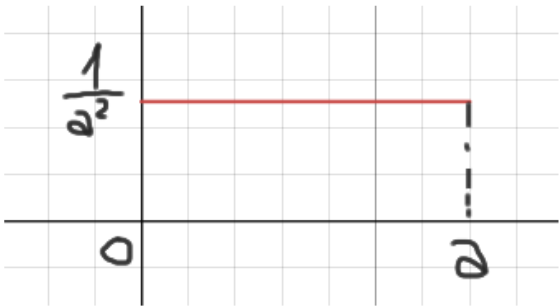
\includegraphics[scale=0.6]{03-TransformadaDeLaplace/3a1.png}
    
    Mirando esto, podemos sacar partido de la función escalón unitario, y redefinir a la función en términos de ella:
    
    $\displaystyle y(t)=\frac{1}{a^{2}}E(t)-\frac{1}{a^{2}}E(t-a)$
    
    Básicamente, lo que estamos haciendo es multiplicar a nuestra función por una función escalón unitario, lo cual nos daría todo el trozo que corresponde a su dominio, y luego, le restamos la parte que no consideramos (ya que para valores mayores a $a$, la función es 0).
    
    Algo a considerar es que no hace falta ``restar'' la parte de $t<0$, ya que la función escalón unitario está definida para $t \geq 0$.
    
    Luego, transformamos la función que tenemos. 
    
    \textbf{\underline{NOTA:}} 
    
    $\displaystyle \lapl{E(t)}=\frac{1}{s}$
    
    $\displaystyle \lapl{E(t-a)}=\frac{e^{-as}}{s}$
    
    $\displaystyle \lapl{y(t)}=\frac{1}{a^{2}} \cdot \frac{1}{s}- \frac{1}{a^{2}} \cdot \frac{e^{-as}}{s} \implies$
    \fcolorbox{black}{yellow}{$\displaystyle Y(s)=\frac{1-e^{-as}}{a^{2}s}$}
    
    \subsubsection{3b}
    $y(t)=\sen \left(5t+\frac{\pi}{3} \right)\;;\;t>0$
    
    Para resolver este ejercicio, hay que darse cuenta que no se puede aplicar la segunda propiedad de la traslación, ya que no se cumplen las condiciones para poder aplicarla.
    
    Resulta, entonces, que hay que hacer un paso extra para poder transformar esta función. En este caso, basta con aplicar el seno de la suma:
    
    $\displaystyle y(t)=\sen \left(5t\right)\cdot \cos\left(\frac{\pi}{3}\right)+ \sen\left(\frac{\pi}{3}\right)\cdot\cos\left(5t\right)$
    
    Calculamos los números: $\displaystyle y(t)=\frac{1}{2}\sen(5t)+\frac{\sqrt{3}}{2}cos(5t)$
    
    Transformamos usando la tabla: $\displaystyle Y(s)=\frac{1}{2}\frac{5}{s^{2}+25}+\frac{\sqrt{3}}{2}\frac{s}{s^{2}+25}\implies$ \fcolorbox{black}{yellow}{$\displaystyle Y(s)=\frac{\sqrt{3}s+5}{2\left(s^{2}+25\right)}$}
    
    \subsubsection{3c}
    $y(t)=\cos^{3}(t)$
    
    Se puede proceder de muchas maneras para resolver este ejercicio. Yo voy a optar por transformar esta expresión en una equivalente.
    
    Si usamos la forma exponencial del coseno: (recordar) $\displaystyle cos(a)=\frac{e^{aj}+e^{-aj}}{2}$
    
    $\displaystyle y(t)=\left(\frac{e^{jt}+e^{-jt}}{2}\right)^{3}
    =\frac{e^{3jt}}{8}+\frac{3e^{2jt}\cdot e^{-jt}}{8}+\frac{3e^{jt}\cdot e^{-2jt}}{8}+\frac{e^{-3jt}}{8}$
    
    Operando, ordenando y agrupando convenientemente: $\displaystyle y(t)=
    \frac{\highlight{yellow}{ e^{3jt}+e^{-3jt}}}{\highlight{yellow}{2}\cdot4}+\frac{3\left( \highlight{green}{e^{jt}+e^{-jt}} \right)} {\highlight{green}{2}\cdot4}$
    
    Si nos damos cuenta, lo sombreado con amarillo y con verde, representan también la forma exponencial de un coseno, entonces, lo reemplazamos:
    
    $\displaystyle y(t)=\frac{1}{4}\cos(3t)+\frac{3}{4}\cos(t)$
    
    Ahora, estamos en condiciones de transformar directamente: \fcolorbox{black}{yellow}{$\displaystyle Y(s)=\frac{1}{4}\cdot \frac{s}{s^{2}+9}+\frac{3}{4}\cdot \frac{s}{s^{2}+1}$}
    
    \subsubsection{3d}
    $y(t)=a^{t} \; ; \; t>0 \; ; \; a \in \mathbb{R}^{+}$
    
    Aplicamos logaritmo a ambos miembros
    
    $\ln(y(t))=t \ln(a)$
    
    $ \displaystyle e^{\ln(y(t))}=e^{t\cdot ln(a)} \implies y(t)=e^{\ln(a)t}$
    
    ¡Que no panda el cúnico! el $\ln(a)$ es un número! Entonces, podemos transformar directamente usando la tabla para la exponencial:
    
    \fcolorbox{black}{yellow}{$\displaystyle Y(s)=\frac{1}{s-\ln(a)}$}
    
    \subsubsection{3e}
    $y(t)=(t-1)^{4} \; ; \; t>0$
    
    Este ejercicio es una variante del ejercicio 2d. ¿Cuál es la diferencia? El dominio donde está definida la función. Para el ejercicio 2d, decía claramente $t>1$, de forma tal que podíamos aplicar la segunda propiedad de la traslación.
    
    En este caso, no coincide el desplazamiento de la función, con el dominio. Por ende, no se cumplen las hipótesis para aplicar la propiedad.
    
    ¿Qué hacemos? Desarrollamos el binomio y transformamos el resultado. Entonces:
    
    $y(t)=t^{4}-4t^{3}+6t^{2}-4t+1$
    
    $\displaystyle \lapl{y(t)}=\frac{4!}{s^{5}}-4\frac{3!}{s^{4}}+6\frac{2!}{s^{3}}-4\frac{1!}{s^{2}}+\frac{1}{s}$
    
    \fcolorbox{black}{yellow}{$\displaystyle Y(s)=\frac{24}{s^{5}}-\frac{24}{s^{4}}+\frac{12}{s^{3}}-\frac{4}{s^{2}}+\frac{1}{s}$}
	
	\subsubsection{3f}
	$y(t)=\sen(5t)\cos(2t)\;;\;t>0$
	
	Para este último ejercicio no tenemos una transformada directa. Entonces,toca aplicar alguna identidad trigonométrica, ya que tenemos un seno y un coseno.
	
	Tengamos en cuenta: \fcolorbox{black}{white}{$\displaystyle \sen(a)\cdot \cos(b) = \frac{\sen(a-b)+\sen(a+b)}{2}$}
	
	Usamos la identidad:
	$\displaystyle y(t)=\frac{1}{2}\sen(5t-2t)+\frac{1}{2} \sen(5t+2t)$
	
	$\displaystyle y(t)=\frac{1}{2}\sen(3t)+\frac{1}{2} \sen(7t)$
	
	Estas dos funciones ya son transformables:
	
	$\displaystyle Y(s)=\frac{3}{2(s^{2}+9)}+\frac{7}{2(s^{2}+49)}=\frac{3(s^{2}+49)+7(s^{2}+9)}{2(s^{2}+9)(s^{2}+49)}=\frac{3s^2+147+7s^2+63}{2(s^2+9)(s^2+49)}$
	
	Por último: \fcolorbox{black}{yellow}{$\displaystyle Y(s)=\frac{5s^2+105}{(s^2+49)(s^2+9)}$}
	
	\subsection{Ejercicio 4}
	Sea $\displaystyle f(t)=k\sen\left(2t+\frac{\pi}{6}\right)$. Determine el valor de $k$ sabiendo que $\lim\limits_{s \rightarrow \infty} sF(s)=4$.\\
	Recuerde el teorema de valor inicial.
	
	Tal como sugiere el ejercicio, debemos aplicar el teorema de valor inicial. ¿Qué nos decía?
	
	Decía que: $\lim\limits_{t \rightarrow 0} f(t)=\lim\limits_{s \rightarrow \infty}sF(s)$
	
	A nosotros nos están dando como dato el miembro derecho de la igualdad. Entonces queda calcular el límite del miembro izquierdo.
	
	$\displaystyle \lim\limits_{t \rightarrow 0}k\sen\left(2t+\frac{\pi}{6}\right)=4 \implies k\cdot\sen\left(\frac{\pi}{6}\right)=4 \implies k\cdot \frac{1}{2}=4 \implies$
	\fcolorbox{black}{yellow}{$k=8$}
	
	\section{Parte 2: Antitransformada de Laplace - Propiedades}
	\subsection{Ejercicios 5afg}
	Calcule las Antitransformadas de Laplace de las siguientes funciones.
	
	\subsubsection{5a}
	$\displaystyle Y(s)=\frac{25}{s^{3}}$
	
	Para los ejercicios de Antitransformada, siempre hay que mirar la tabla de transformadas, pero ``al revés''. Es muy parecido a como hicimos para las transformadas. A veces puede darse el caso en que necesitemos hacer algún paso algebráico o, como vamos a ver en el ejercicio 6, aplicar fracciones simples.
	
	Para este caso, primero aplicamos linealidad, y luego hacemos la antitransformada directa:
	
	$\displaystyle \ilapl{Y(s)}=25\ilapl{\frac{1}{s^{3}}}$
	
	Por definición, $\ilapl{Y(s)}=y(t)$. Luego, para antitransformar la otra función, necesitamos un $2$ en el numerador. Como no lo tenemos, lo generamos y luego compensamos:
	
	$\displaystyle y(t)=\frac{25}{2}\ilapl{\frac{2}{s^{3}}} \implies$ \fcolorbox{black}{yellow}{$\displaystyle y(t)=\frac{25}{2}t^{2}$}
	
	\subsubsection{5f}
	$\displaystyle Y(s)=\frac{s+3}{s^{2}+6s+13}$
	
	Esta función si la observamos minuciosamente se puede asemejar (aunque no es igual) a un coseno transformado.
	
	En el denominador, podemos llegar a formar un trinomio cuadrado perfecto. Tenemos el $s^{2}$ y el $6s$, el término independiente es incorrecto.
	
	Si no te acordás como formarlo, una ayudita rápida:
	
	Tomamos el coeficiente del término lineal: $6$, y lo dividimos entre $2$: $\frac{6}{2}=3$. A este resultado, lo elevamos al cuadrado $3^{2}=\boxed{9}$
	
	Este último número es el que debemos usar para tener un trinomio cuadrado perfecto. Entonces, para obtenerlo, vamos a separar el término independiente del denominador en $9+4$:
	
	$\displaystyle Y(s)=\frac{s+3}{s^{2}+6s+9+4}=\frac{s+3}{(s+3)^{2}+4}$
	
	Ahora sí, esto se parece mucho más a un coseno, lo que tiene es que está desplazado. ¿Te acordás que propiedad genera un desplazamiento en el dominio de Laplace?
	
	Pensalo 3 segundos...
	3...\\
	2...\\
	1...\\
	
	¡Si! La \textbf{primera propiedad de la traslación}. Ahora, la tenemos que aplicar a la inversa.
	
	\textbf{ATENCIÓN, IMPORTANTE!!!!!:} para poder aplicar la propiedad, en el caso del coseno necesitamos que \textbf{\underline{TODAS}} las $s$ estén desplazadas. Es decir, que si tengo: $\displaystyle Y(s)=\frac{s}{(s+3)^{2}+4}$ no podríamos aplicar la propiedad, en principio. Tendríamos que aplicar una serie de pasos algebraicos adicionales (ya tendremos la oportunidad de hacerlos, en este caso, está hecho a propósito).
	
	Dicho esto, antitransformamos. El tip que va a servirte es que antitransformemos haciendo de cuenta que en vez de $s+3$ tenemos $s$, y luego, en el dominio del tiempo hacemos la corrección que haga falta.
	
	$\displaystyle \ilapl{Y_{2}(s)}=\ilapl{\frac{s}{s^{2}+4}} \implies y_{2}(t)=\cos(2t)$
	
	Para obtener la $y(t)$, multiplicamos por la exponencial de la propiedad: \fcolorbox{black}{yellow}{$y(t)=e^{-3t}\cos(2t)$}
	
	\subsubsection{5g}
	$\displaystyle Y(s)=\frac{s-1}{s^{2}+2s+2}$
	
	Este ejercicio va a servir para poner en ejemplo la advertencia que hicimos en el anterior.
	
	Vamos primero a armar el trinomio cuadrado perfecto del denominador:
	
	$\displaystyle Y(s)=\frac{s-1}{s^{2}+2s+1+1}=\frac{s-1}{(s+1)^{2}+1}$.
	
	En este caso, vemos que no coinciden las ``s'', ya que una es $s+1$ y la otra $s-1$. No podemos aplicar la propiedad (directamente).
	
	Entonces, vamos a hacer una jugarreta. En el numerador sumamos y restamos 1:
	
	$\displaystyle Y(s)=\frac{s-1+1-1}{(s+1)^{2}+1} \;\;\;$. Agrupamos convenientemente: $\displaystyle Y(s)=\frac{s+1-2}{(s+1)^{2}+1}$
	
	Distribuyendo: $\displaystyle Y(s)=\frac{s+1}{(s+1)^2+1}-\frac{2}{(s+1)^2+1}$
	
	Y ahora si, podemos antitransformar directamente, considerando la traslación como hicimos en el ejercicio anterior:
	
	\fcolorbox{black}{yellow}{$y(t)=\cos(t)e^{-t}-2\sen(t)e^{-t}$}
	
	\subsection{Ejercicios 6abij}
	Calcule las Antitransformadas de Laplace de las siguientes funciones previamente separando en fracciones simples.
	
	\subsubsection{6a}
	$\displaystyle F(s)=\frac{s+7}{s^2-6s+5}$
	Para resolver estos ejercicios, como nos dice el enunciado, debemos separar en fracciones simples.
	
	Para hacer eso, se procede a factorizar el denominador. Luego, el planteo varía según el ejercicio.
	
	Consideremos el siguiente cociente: $\frac{P(x)}{Q(x)}$
	
	La primera condición que tenemos que verificar es que el \textbf{$gr(P(x)) < gr(Q(x))$}
	
	Luego, hay que hacer un análisis de distintos casos que nos pueden aparecer.
	
	\textit{1)} \textbf{Si $Q(x)$ tiene raíces reales distintas}
	
	$\displaystyle \frac{P(x)}{Q(x)}=\frac{A}{x-\alpha}+\frac{B}{x-\beta}+...+\frac{H}{x-\gamma}$
	
	\textit{2)} \textbf{Si $Q(x)$ tiene raíces reales múltiples}
	
	$\displaystyle \frac{P(x)}{(x-\alpha)^n}=\frac{A}{(x-\alpha)^{n}}+\frac{B}{(x-\alpha)^{n-1}}+...+\frac{H}{x-\alpha}$
	
	\textit{3)} \textbf{Si $Q(x)$ tiene raíces complejas conjugadas}
	
	$\displaystyle \frac{P(x)}{ax^2+bx+c}=\frac{Ax+B}{ax^2+bx+c} \;\; ; \; \; b^2-4ac<0$
	
	\textit{4)} \textbf{Si $Q(x)$ tiene raíces complejas conjugadas múltiples} (el peor caso)
	
	$\displaystyle \frac{P(x)}{(ax^2+bx+c)^n}=\frac{Ax+B}{(ax^2+bx+c)^n}+\frac{Cx+D}{(ax^2+bx+c)^{n-1}}+...+\frac{Hx+I}{ax^2+bx+c}\;\; ; \; \; b^2-4ac<0$
	
	Con toda esta teoría planteada, vamos a resolver el ejercicio en cuestión.
	
	Vemos que cumple la condición del grado, y es un ejercicio del tipo 1). Factorizamos el denominador:
	
	$\displaystyle F(s)=\frac{s+7}{s^2-6s+5}=\frac{s+7}{(s-5)(s-1)}$
	
	Planteamos las fracciones simples:
	\\ $\displaystyle \frac{s+7}{(s-5)(s-1)}=\frac{A}{s-5}+\frac{B}{s-1}$
	
	Tenemos que resolver para $A$ y para $B$:
	
	$s+7=A(s-1)+B(s-5) \implies s+7=As-A+Bs-5B$
	
	Para que esta igualdad se cumpla, deben ser iguales los dos miembros coeficiente a coeficiente:
	
	Para las $s$:\\
	$1=A+B \rightarrow \boxed{B=1-A} \;\;\;\; \circled{1}$
	
	Para los términos independientes:\\
	$7=-A-5B \rightarrow \mathrm{Aplicando\; \circled{1}} \rightarrow 7=-A-5(1-A)\rightarrow 7=-A-5+5A \rightarrow 12=4A \rightarrow \boxed{A=3}$
	
	Reemplazando el resultado de $A$ en \circled{1} queda: $B=1-3\rightarrow \boxed{B=-2}$
	
	Por lo tanto, nuestra función ya con fracciones simples queda: $\displaystyle F(s)=\frac{3}{s-5}+\frac{-2}{s-1}$
	
	Antitransformando, nos queda finalmente: \fcolorbox{black}{yellow}{$f(t)=3e^{5t}-2e^{t}$}
	\subsubsection{6b}
	$\displaystyle F(s)=\frac{s^{2}+2s+2}{s^{2}+3s+2}$
	
	En este ejercicio tenemos un pequeño problema. No podemos aplicar fracciones simples, debido a que $gr(P(x)) \ge gr(Q(x))$
	
	Para saldar ese problema hay que hacer la división de los polinomios, es decir expresar: \\$\displaystyle \frac{P(x)}{Q(x)}=C(x)+\frac{R(x)}{Q(x)}$
	
	\[
	\begin{array}{r|r}
		\dropsign{-} s^2 + 2s + 2 & s^2 + 3s + 2 \\ \cline{2-2}
		s^2 + 3s + 2 & 1 \\ \cline{1-1} \\[\dimexpr-\normalbaselineskip+\jot]
		-s \phantom{+00}\\
	\end{array}
	\]
	
	Entonces, la función queda expresada:\\
	$\displaystyle F(s)=1 + \frac{-s}{s^2+3s+2} \implies F(s)=1-\frac{s}{(s+1)(s+2)}$
	
	
	Fracciones simples:
	
	$\displaystyle F(s)=1+\frac{A}{s+1}+\frac{B}{s+2} \implies F(s)=1+\frac{1}{s+1}+\frac{-2}{s+2}$
	
	\fcolorbox{black}{yellow}{$\ilapl{F(s)}=f(t)=\delta(t)+e^{-t}-2e^{-2t}$}
	
	\subsubsection{6i}
	$\displaystyle F(s)=\frac{-2s^{2}+8s-14}{(s+1)(s^{2}-2s+5)}$
	
	Procedemos a aplicar fracciones simples, teniendo cuidado de que el segundo factor del denominador tiene raíces complejas:
	
	$\displaystyle \frac{-2s^2+8s-14}{(s+1)(s^2-2s+5)}=\frac{\cancelto{-3}{A}}{s+1}+\frac{Bs+C}{s^2-2s+5}$
	
	$\displaystyle -2s^2+8s-14=-3(s^2-2s+5)+(Bs+C)(s+1)$\\
	$\displaystyle -2s^2+8s-14=-3s^2+6s-15+Bs^2+Bs+Cs+C$
	
	Igualamos grado a grado:\\
	$-2=-3+B \rightarrow B=1$\\
	$8=6+B+C \rightarrow 8=6+1+1 \rightarrow \text{Verifica}$\\
	$-14=-15+C \rightarrow C=1$
	
	Queda, entonces, nuestra $F(s)$ como:
	
	$\displaystyle F(s)=\frac{-3}{s+1}+\frac{s+1}{s^2-2s+5}=\frac{-3}{s+1}+\frac{s+1}{(s-1)^2+4}$
	
	Ahora bien, uno podría decir ``distribuyo el denominador del segundo término'' y antitransformo en consecuencia, es decir, hacer algo así:
	
	$\displaystyle F(s)=\frac{-3}{s+1}+\frac{s+1}{s^2-2s+5}=\frac{-3}{s+1}+\frac{s}{(s-1)^2+4}+\frac{1}{(s-1)^2+4}$
	
	Sin embargo, hacer esto es un gran error, y uno bastante común, de hecho. El segundo término de la expresión de aquí arriba debe tener a todas las $s$ trasladadas, es decir, que para poder antitransformar sin problemas en el numerador debería decir $s-1$.
	
	Entonces, ¿qué hacemos? Si! Restamos y sumamos un uno ;). Volviendo a la expresión original:
	
	$\displaystyle F(s)=\frac{-3}{s+1}+\frac{s+1}{s^2-2s+5}=\frac{-3}{s+1}+\frac{s+1+1-1}{(s-1)^2+4}$
	
	Agrupamos convenientemente:
	
	$\displaystyle F(s)=\frac{-3}{s+1}+\frac{s+1}{s^2-2s+5}=\frac{-3}{s+1}+\frac{s-1+2}{(s-1)^2+4}$
	
	Ahora si, distribuimos:
	
	$\displaystyle F(s)=\frac{-3}{s+1}+\frac{s+1}{s^2-2s+5}=\frac{-3}{s+1}+\frac{s-1}{(s-1)^2+4}+\frac{2}{(s-1)^2+4}$
	
	Antitransformamos y obtenemos la respuesta:
	
	\fcolorbox{black}{yellow}{$\displaystyle f(t)=-3e^{-t}+\cos(2t)e^t+\sen(2t)e^t$}
	
	\subsubsection{6j}
	$\displaystyle F(s)=\frac{(4s+2)e^{-2s}}{(s-1)(s+2)}$
	
	Este ejercicio tiene de distinto que tenemos una ¿¿exponencial?? ¿¿¿en el dominio de Laplace???
	
	¿Hay algo que está mal? No! Simplemente es una función que en el dominio del tiempo estaba desplazada, y se le tuvo que aplicar la segunda propiedad de la traslación.
	
	Para resolverlo, hay que obviar a la exponencial, por ahora, y calcular fracciones simples sobre lo demás:
	
	$\displaystyle \frac{4s+2}{(s-1)(s+2)}=\frac{\cancelto{2}{A}}{s-1}+\frac{\cancelto{2}{B}}{s+2}$
	
	Una vez que calculamos las fracciones simples, vamos a devolver la exponencial a los dos términos:
	
	$\displaystyle F(s)=\frac{2e^{-2s}}{s-1}+\frac{2e^{-2s}}{s+2}$
	
	Para antitransformar esto lo que hacemos es, otra vez, ignorar a la exponencial, antitransformar como si no estuviera, y luego aplicamos la segunda propiedad de la traslación:
	
	$\ilapl{F_{1}(s)}=f_{1}(t)=2e^t+2e^{-2t}$
	
	Ahora, aplicamos la traslación, considerando que esta se hace en $t$:
	
	\fcolorbox{black}{yellow}{$f(t)=2e^{t-2}+2e^{-2(t-2)}$}
	
	\section{Parte 3: Resolución de ecuaciones diferenciales}
	\subsection{Ejercicios 8egi}
	Resuelva las siguientes Ecuaciones Diferenciales por Transformada de Laplace:
	\subsubsection{8e}
	$y''(t)+4y'(t)+4y(t)=3x'(t)+2x(t) \;\;\;\;\; \mathrm{con} \; x(t)=e^{-5t} \wedge y(0)=0 \wedge y'(0)=0$
	
	Para resolver estos ejercicios, la estrella es la propiedad de ``Transformada de Laplace de las derivadas''.
	
	Pero primero, nos dan el dato de $x(t)$, que podemos reemplazar.\\
	Calculemos $x'(t)$
	
	$x'(t)=-5e^{-5t}$
	
	Reemplazamos esto en nuestra ecuación:
	
	$y''(t)+4y'(t)+4y(t)=3\left(-5e^{-5t}\right)+2e^{-5t} \rightarrow \boxed{y''(t)+4y'(t)+4y(t)=-13e^{-5t}}$
	
	Transformamos:
	
	$\displaystyle s^2Y(s)-sy(0)-y'(0)+4sY(s)-y(0)+4Y(s)=\frac{-13}{s+5}$
	
	$\displaystyle s^2Y(s)-\cancelto{0}{sy(0)}-\cancelto{0}{y'(0)}+4sY(s)-\cancelto{0}{y(0)}+4Y(s)=\frac{-13}{s+5}$
	
	$\displaystyle Y(s)\left(s^2+4s+4\right)=\frac{-13}{s+5}$
	
	Ahora, despejamos nuestra función objetivo $Y(s)$:
	
	$\displaystyle Y(s)=\frac{-13}{(s+5)(s^2+4s+4)}$
	
	El siguiente paso en estos ejercicios es antitransformar la función que despejamos. En este caso, debemos aplicar fracciones simples:
	
	$\displaystyle Y(s)=\frac{-13}{(s+5)(s+2)^{2}}$
	
	$\displaystyle \frac{-13}{(s+5)(s+2)^2}=\frac{A}{s+5}+\frac{B}{(s+2)^2}+\frac{C}{s+2}$
	
	Resolviendo: $\displaystyle A=\frac{-13}{9}\;\;\;;B=\frac{-13}{3}\;\;\;;C=\frac{13}{9}\;\;\;$
	
	$\displaystyle Y(s)=\frac{-\frac{13}{9}}{s+5}+\frac{-\frac{13}{3}}{(s+2)^2}+\frac{\frac{13}{9}}{s+2}$
	
	\fcolorbox{black}{yellow}{$\displaystyle y(t)=-\frac{13}{9}e^{-5t}-\frac{13}{3}te^{-2t}+\frac{13}{9}e^{-2t}$}
	
	\subsubsection{8g}
	$y''(t)-2y'(t)+5y(t)=-8e^{-t} \;\;\;\;\; \mathrm{con} \; y(0)=2 \wedge y'(0)=12$
	
	Transformamos:
		
	$\displaystyle s^2Y(s)-s\cancelto{2}{y(0)}-\cancelto{12}{y'(0)}-2sY(s)+2\cancelto{2}{y(0)}+5Y(s)=-\frac{-8}{s+1}$
	
	$\displaystyle Y(s)(s^2-2s+5)-2s-12+4=\frac{-8}{s+1}$
	
	$\displaystyle Y(s)(s^2-2s+5)=\frac{-8}{s+1}+2s+8$
	
	$\displaystyle Y(s)=\frac{2s^2+10s}{(s+1)(s^2-2s+5)}$
	
	Ahora, aplicamos fracciones simples:
	
	$\displaystyle \frac{2s^2+10s}{(s+1)(s^2-2s+5)}=\frac{\cancelto{-1}{A}}{s+1}+\frac{Bs+C}{s^2-2s+5}$
	
	$\displaystyle 2s^2+10s=-s^2+2s-5+Bs^2+Bs+Cs+C$
	
	$\displaystyle 2=-1+B \rightarrow \boxed{B=3}$ \\
	$\displaystyle 10=2+B+C \rightarrow \mathrm{Verifica}$ \\
	$\displaystyle 0=-5+C$ $\rightarrow \boxed{C=5}$
	
	$\displaystyle Y(s)=\frac{-1}{s+1}+\frac{3s+5}{s^2-2s+5}=\frac{-1}{s+1}+\frac{3s+5}{\boxed{s^2-2s+1}+4}=\frac{-1}{s+1}+\frac{3s+5}{(s-1)^2+4}$
	
	Para poder antitransformar esta función, primero debemos resolver el $s-1$ del segundo término, para eso, sumamos y restamos un uno en el numerador:
	
	$\displaystyle \frac{3(s-1+1)+5}{(s-1)^2+4}=\frac{3(s-1)+3+5}{(s-1)^2+4}=\frac{3(s-1)}{(s-1)^2+4}+\frac{8}{(s-1)^2+4}$
	
	$\displaystyle Y(s)=\frac{-1}{s+1}+\frac{3(s-1)}{(s-1)^2+4}+4\frac{2}{(s-1)^2+4}$
	
	Ahora si, podemos antitransformar:
	
	\fcolorbox{black}{yellow}{$\displaystyle y(t)=-e^{-t}+3\cos(2t)e^t+4\sen(2t)e^t$}
	
	\subsubsection{8i}
	$\displaystyle y''(t)+9y(t)=\cos(2t) \;\;\;\;\; \mathrm{con} \; y(0)=1 \wedge y\left(\frac{\pi}{2}\right)=-1$
	
	Transformamos:
	
	$\displaystyle s^2Y(s)-s\cancelto{1}{y(0)}-y'(0)+9Y(s)=\frac{s}{s^2+4}$
	
	Llamamos $y'(0)=k$
	
	$\displaystyle Y(s)(s^2+9)=\frac{s}{s^2+4}+s+k$
	
	$\displaystyle Y(s)=\frac{s^3+ks^2+5s+4k}{(s^2+4)(s^2+9)}$
	
	Aplicamos fracciones simples:
	
	$\displaystyle \frac{s^3+ks^2+5s+4k}{(s^2+4)(s^2+9)}=\frac{As+B}{s^2+4}+\frac{Cs+D}{s^2+9}$
	
	$s^3+ks^2+5s+4k=As^3+Bs^2+9As+9B+Cs^3+Ds^2+4Cs+4D$
	
	$1=A+C \;\; \circled{1}$\\
	$k=B+D \;\;\circled{2}$\\
	$5=9A+4C \;\;\circled{3}$\\
	$4k=9B+4D \;\;\circled{4}$\\
	
	De \circled{1}:\\ $1-A=C$
	
	En \circled{3}:\\ $\displaystyle 5=9A+4(1-A) \rightarrow 5=9A+4-4A \rightarrow 5=5A+4 \rightarrow \boxed{A=\frac{1}{5}}$
	
	En \circled{1}: $1-\frac{1}{5}=C \rightarrow \boxed{C=\frac{4}{5}}$
		
	Luego, de \circled{2}: \\$k-B=D$
	
	En \circled{4}: \\$4k=9B+4(k-B) \rightarrow 4k=9B+4k-4B \rightarrow 0=5B \rightarrow \boxed{B=0}$
	
	De donde $k-B=D \rightarrow \boxed{k=D}$
	
	Entonces, $\displaystyle Y(s)=\frac{\frac{1}{5}s}{s^2+4}+\frac{\frac{4}{5}s+k}{s^2+9}=\frac{\frac{1}{5}s}{s^2+4}+\frac{\frac{4}{5}s}{s^2+9}+\frac{k}{3}\cdot\frac{3}{s^2+9}$
	
	Antitransformamos:
	
	$\displaystyle y(t)=\frac{1}{5}\cos(2t)+\frac{4}{5}\cos(3t)+\frac{k}{3}\sen(3t)$
	
	Ahora, usamos el dato $\displaystyle y\left(\frac{\pi}{2}\right)=-1$
	
	$\displaystyle -1=\frac{1}{5}\cos\left(2 \cdot \frac{\pi}{2}\right)+\frac{4}{5}\cos\left(3 \cdot \frac{\pi}{2}\right)+\frac{k}{3}\sen\left(3 \cdot \frac{\pi}{2}\right)$
	
	$\displaystyle -1=-\frac{1}{5}+0-\frac{k}{3} \rightarrow \boxed{k=\frac{12}{5}}$
	
	Por último: \fcolorbox{black}{yellow}{$\displaystyle y(t)=\frac{1}{5}\cos(2t)+\frac{4}{5}\cos(3t)+\frac{4}{5}\sen(3t)$}
	
	\subsection{Ejercicio 9}
	Resuelva los siguientes Sistemas de Ecuaciones Diferenciales por medio de la Transformada de Laplace:
	\subsubsection{9d}
	$\begin{cases}
		x'(t) + 2y'(t)+5x(t)= & 0  \\
		y'(t) +y(t)+2x(t)= & 0
	\end{cases}$ $\;\;\;\;\mathrm{con} \; y(0)=1 \wedge x(0)=0$

	Para resolver estos ejercicios, se procede casi de la misma manera que para las ecuaciones diferenciales del ejercicio 8. Primero, transformamos ambas ecuaciones:
	
	$\begin{cases}
		sX(s)-x(0)+2sY(s)-2y(0)+5X(s)=0 \\
		sY(s)-y(0)+Y(s)+2X(s)=0
	\end{cases}$

	$\begin{cases}
		sX(s)+2sY(s)-2+5X(s)=0 \\
		sY(s)-1+Y(s)+2X(s)=0
	\end{cases}$

	Ordenamos el sistema: \\
	$\begin{cases}
		(s+5)X(s)+2sY(s)=2 \\
		2X(s)+(s+1)Y(s)=1
	\end{cases}$

	Ahora, para resolver el sistema, podemos usar la regla de Cramer. Hallemos los determinantes:
	
	$\Delta = \begin{vmatrix}
		s+5 & 2s \\
		2 & s+1
	\end{vmatrix} = (s+5)\cdot(s+1)-2s\cdot 2=s^2+2s+5=(s+1)^2+4$

	$\Delta X(s) = \begin{vmatrix}
		2 & 2s \\
		1 & s+1
	\end{vmatrix}= 2(s+1)-2s = 2$

	$\Delta Y(s) = \begin{vmatrix}
		s+5 & 2 \\
		2 & 1
	\end{vmatrix}=s+5-4=s+1$

	Luego, $\displaystyle X(s)=\frac{\Delta X(s)}{\Delta}$ y $\displaystyle Y(s)=\frac{\Delta Y(s)}{\Delta}$
	
	Entonces, si expresamos según la regla:
	
	$\displaystyle X(s)=\frac{2}{(s+1)^2+4}$
	
	$\displaystyle Y(s)=\frac{s+1}{(s+1)^2+4}$
	
	Por último, se antitransforman estas expresiones, y se llega a la solución:
	
	\fcolorbox{black}{yellow}{$x(t)=\sen(2t)e^{-t} \;\;;\;\; y(t)=\cos(2t)e^{-t}$}
	
	\section{Parte 4: Convolución}
	\subsection{Ejercicio 10}
	Halle $\displaystyle \lapl{\int_{0}^{t}u\cos(u)e^{t-u}du}$ utilizando el Teorema de Convolución.
	
	Recordemos el Teorema de Convolución:
	
	Si $\displaystyle f(t)=\ilapl{F(s)} \wedge g(t)=\ilapl{G(s)} \implies \ilapl{F(s) \bullet G(s)}=\int_{0}^{t}f(u)g(t-u)du$
	
	O bien, podemos verlo al revés: $\displaystyle \lapl{\int_{0}^{t}f(u)g(t-u)du}=F(s) \bullet G(s)$
	
	Esta última es la que tenemos que usar:
	
	Usamos: $f(t)=tcos(t)$ y $g(t)=e^{t}$
	
	Calculamos las transformadas: $\displaystyle \lapl{f(u)}=(-1)\left(\frac{s}{s^2+1}\right)'=(-1)\frac{s^2+1-2s^2}{(s^2+1)^2}= \dots$\\
	$\displaystyle \dots = \frac{s^2-1}{(s^2+1)^2} \implies F(s)=\frac{(s+1)(s-1)}{(s^2+1)^2}$
	
	$\displaystyle \lapl{g(t)}=\frac{1}{s-1}$
	
	Ahora, usando la definición del Teorema de Convolución: $\displaystyle F(s) \bullet G(s) = \frac{(s+1)(s-1)}{(s^2+1)^2}\cdot \frac{1}{s-1}$
	
	Quedando: \fcolorbox{black}{yellow}{$\displaystyle F(s)\bullet G(s)=\frac{s+1}{(s^2+1)^2}$}
	
	\subsection{Ejercicio 11}
	Antitransforme utilizando Convolución:
	\subsubsection{11b}
	$\displaystyle Y(s)=\frac{1}{(s^2+1)^2}$
	
	Para este ejercicio, debemos aplicar el teorema al revés de como lo aplicamos en el ejercicio 10. Hay que dividir a la función en otras dos, para que podamos usar el teorema:
	
	$\displaystyle F(s)=\frac{1}{s^2+1}$ y $\displaystyle G(s)=\frac{1}{s^2+1}$
	
	Ahora, aplicamos la definición:\\
	$\displaystyle \ilapl{F(s)\bullet G(s)}= \int_{0}^{t}\sen(u)\sen(t-u)du$
	
	Usamos la identidad trigonométrica: $\displaystyle \sen(x)\sen(y)=\frac{\cos(x-y)-\cos(x+y)}{2}$
	
	$\displaystyle \ilapl{F(s)\bullet G(s)}= \frac{1}{2} \int_{0}^{t}(\cos(u-t+u)-\cos(u+t-u))du=\frac{1}{2}\int_{0}^{t}(\cos(2u-t)-\cos(t))du = \dots$
	
	$\displaystyle \dots = \frac{1}{2} \left[\frac{\sen(2u-t)}{2}-u\cos(t)\right]_{0}^{t}=\frac{1}{2}\left[\frac{\sen(t)}{2}-\frac{\sen(-t)}{2}-t\cos(t)\right]$
	
	Operando, llegamos a:
	
	\fcolorbox{black}{yellow}{$\displaystyle \ilapl{F(s)\bullet G(s)}=\frac{1}{2}\sen(t)-\frac{1}{2}t\cos(t)$}
	
	\subsection{Ejercicios 12bdef}
	Resuelva las siguientes ecuaciones integrales e integrodiferenciales por medio de la Transformada de Laplace, utilizando el Teorema de Convolución
	\subsubsection{12b}
	$\displaystyle y(t)=t+2\int_{0}^{t}\cos(t-u)y(u)du$
	
	Para esta serie de ejercicios, vamos a usar el Teorema de Convolución de la forma que lo usamos en el ejercicio 10.
	
	Se procede de la misma manera que para la resolución de ecuaciones diferenciales. Primero se transforma, se agrupa en $Y(s)$, luego, se trabaja la expresión en el dominio de Laplace, y luego antitransformamos para obtener la solución temporal.
	
	Transformamos:
	
	$\displaystyle Y(s)=\frac{1}{s^2}+ \frac{2s}{s^2+1}\cdot Y(s)$
	
	Intentamos agrupar para $Y(s)$
	
	$\displaystyle Y(s)-\frac{2s}{s^2+1}Y(s)=\frac{1}{s^2} \rightarrow Y(s)\left(1-\frac{2s}{s^2+1}\right)=\frac{1}{s^2} \rightarrow Y(s)\left(\frac{s^2-2s+1}{s^2+1}\right)=\frac{1}{s^2}$
	
	$\displaystyle Y(s)=\frac{s^2+1}{s^2(s^2-2s+1)}=\frac{s^2+1}{s^2(s-1)^2}$
	
	Toca el turno de aplicar fracciones simples:
	
	$\displaystyle \frac{s^2+1}{s^2(s-1)^2}=\frac{\cancelto{1}{A}}{s^2}+\frac{B}{s}+\frac{\cancelto{2}{C}}{(s-1)^2}+\frac{D}{s-1}$
	
	$s^2+1=(s-1)^2+Bs(s-1)^2+2s^2+D(s-1)s^2$\\
	$s^2+1=s^2-2s+1+Bs^3-2Bs^2+Bs+2s^2+Ds^3-Ds^2$
	
	$0=B+D \; \circled{1}$\\
	$1=1-2B+2-D \; \circled{2}$\\
	$0=-2+B \; \circled{3}$\\
	$1=1 \rightarrow \mathrm{Verifica}$
	
	De \circled{3}: $B=2$\\
	En \circled{1}: $D=-2$
	
	$B$ y $D$ en \circled{2}: $1=1-2\cdot 2 + 2 - (-2) \rightarrow 1=1 \rightarrow \mathrm{Verifica}$
	
	Queda entonces nuestra $Y(s)$:
	
	$\displaystyle Y(s)=\frac{1}{s^2}+\frac{2}{s}+\frac{2}{(s-1)^2}+\frac{-2}{s-1}$
	
	Antitransformando:
	
	\fcolorbox{black}{yellow}{$\displaystyle y(t)=t+2+2te^t-2e^t$}
	
	\subsubsection{12d}
	$\displaystyle y(t)=\int_{0}^{t}y(u)du+\cos(t)$
	
	Para este ejercicio, es muy común equivocarse e intentar aplicar el Teorema de Convolución sobre el primer término del segundo miembro. Sin embargo, esa integral puede resolverse fácilmente usando la propiedad de la ``Transformada de Laplace de las Integrales''. Recordémosla:
	
	Si $\displaystyle F(s)=\lapl{f(t)} \implies \lapl{\int_{0}^{t}f(u)du}=\frac{F(s)}{s}$
	
	Teniendo en cuenta esto, transformamos:
	
	$\displaystyle Y(s)=\frac{Y(s)}{s}+\frac{s}{s^2+1} \rightarrow Y(s)-\frac{Y(s)}{s}=\frac{s}{s^2+1}$
	
	Agrupamos en $Y(s)$:
	
	$\displaystyle Y(s)\left(1- \frac{1}{s} \right)=\frac{s}{s^2+1} \rightarrow Y(s)\left(\frac{s-1}{s}\right)=\frac{s}{s^2+1} \rightarrow Y(s)=\frac{s^2}{(s^2+1)(s-1)}$
	
	Aplicamos fracciones simples:
	
	$\displaystyle \frac{s^2}{(s^2+1)(s-1)}=\frac{As+B}{s^2+1}+\frac{\cancelto{\frac{1}{2}}{C}}{s-1}$
	
	$\displaystyle s^2=(As+B)(s-1)+\frac{1}{2}(s^2+1)$\\
	$\displaystyle s^2=As^2-As+Bs-B+\frac{1}{2}s^2+\frac{1}{2}$
	
	$\displaystyle 1=A+\frac{1}{2} \; \circled{1}$\\
	$\displaystyle 0=-A+B \; \circled{2}$\\
	$\displaystyle 0=-B+\frac{1}{2} \; \circled{3}$
	
	De \circled{2}: $A=B$\\
	De \circled{3}: $B=\frac{1}{2} \rightarrow A=\frac{1}{2} \;\; \text{(verifica también en } \circled{1} \mathrm{)}$
	
	Nuestra $Y(s)$ queda:
	
	$\displaystyle Y(s)=\frac{\frac{1}{2}s+\frac{1}{2}}{s^2+1}+\frac{\frac{1}{2}}{s-1}=\frac{\frac{1}{2}s}{s^2+1}+\frac{\frac{1}{2}}{s^2+1}+\frac{\frac{1}{2}}{s-1}$
	
	Antitransformamos:
	
	\fcolorbox{black}{yellow}{$\displaystyle y(t)=\frac{1}{2}\cos(t)+\frac{1}{2}\sen(t)+\frac{1}{2}e^t$}
	
	\subsubsection{12e}
	$\displaystyle \int_{0}^{t}y(u)(t-u)du+y'(t)=\frac{t^4}{12}+t+1 \;\;\;\;\; \text{con }y(0)=-1$
	
	Transformamos:
	
	$\displaystyle Y(s)\cdot \frac{1}{s^2}+sY(s)-\cancelto{-1}{y(0)}=\;\;\frac{1}{\cancel{12}} \cdot \frac{\cancelto{2}{24}}{s^5} + \frac{1}{s^2} + \frac{1}{s}$
	
	$\displaystyle Y(s)\left(\frac{1}{s^2}+s\right)=\frac{2}{s^5}+\frac{1}{s^2}+\frac{1}{s}-1$
	
	$\displaystyle Y(s)\left(\frac{s^3+1}{\cancel{s^{2}}}\right)=\frac{2+s^3+s^4-s^5}{s^{\cancelto{3}{5}}} \rightarrow Y(s)=\frac{2+s^3+s^4-s^5}{s^3(s^3+1)}=\frac{2+s^3+s^4-s^5}{s^3(s+1)(s^2-s+1)}$
	
	Ahora, tocaría aplicar fracciones simples:
	
	$\displaystyle \frac{2+s^3+s^4-s^5}{s^3(s^3+1)}=\frac{A}{s^3}+\frac{B}{s^2}+\frac{C}{s}+\frac{D}{s+1}+\frac{Es+F}{s^2-s+1}$
	
	Calcular estas fracciones simples sería algo MUY tedioso, tenemos 6 incógnitas, de las cuales podemos calcular directamente solo 2, las otras habría que calcularlas haciendo el sistema de ecuaciones.
	
	Para evitar tanto cuenterío, vamos a usar algún artilugio matemático. Vamos a sumar y restar $s^3$ en el numerador:
	
	$\displaystyle Y(s)=\frac{2+s^3+s^3-s^3+s^4-s^5}{s^3(s^3+1)}$
	
	Agrupamos convenientemente: $\displaystyle Y(s)=\frac{2+2s^3-s^3+s^4-s^5}{s^3(s^3+1)}$
	
	Distribuimos convenientemente: $\displaystyle Y(s)=\frac{2+2s^3}{s^3(s^3+1)}+\frac{-s^3+s^4-s^5}{s^3(s^3+1)}$
	
	Sacamos factor común $2$ en el primer término y $-s^3$ en el segundo:\\$\displaystyle Y(s)=\frac{2(1+s^3)}{s^3(s^3+1)}+\frac{-s^3(1-s+s^2)}{s^3(s^3+1)}$
	
	En el segundo miembro, volvemos a factorizar:\\
	$\displaystyle Y(s)=\frac{2\cancel{(1+s^3)}}{s^3\cancel{(s^3+1)}}+\frac{-\cancel{s^3}\cancel{(1-s+s^2)}}{\cancel{s^3}(s+1)\cancel{(s^2-s+1)}}=\frac{2}{s^3}-\frac{1}{s+1}$
	
	Nos quedó una expresión mucho más sencilla, que es muy fácil de antitransformar:
	
	\fcolorbox{black}{yellow}{$y(t)=t^2-e^{-t}$}
	
	\subsubsection{12f}
	$\displaystyle y'(t)=1-\int_{0}^{t}y(u)e^{2(t-u)}du \;\;\;\;\; \mathrm{con}\; y(0)=1$
	
	Este ejercicio tiene todo combinado, es una ecuación integrodiferencial tipo convolutorio. Transformemos:
	
	$\displaystyle sY(s)-\cancelto{1}{y(0)}=\frac{1}{s} - Y(s) \frac{1}{s-2}$
	
	$\displaystyle sY(s)+Y(s) \frac{1}{s-2}=\frac{1}{s} + 1 \rightarrow Y(s)\left(s + \frac{1}{s-2}\right)=\frac{s+1}{s} \rightarrow Y(s)\left(\frac{s^2-2s+1}{s-2}\right) =\frac{s+1}{s}$
	
	$\displaystyle Y(s)=\frac{(s+1)(s-2)}{s(s-1)^2}=\frac{s^2-s-2}{s(s-1)^2}$
	
	Aplicamos fracciones simples:
	
	$\displaystyle \frac{s^2-s-2}{s(s-1)^2}=\frac{\cancelto{-2}{A}}{s}+\frac{\cancelto{-2}{B}}{(s-1)^2}+\frac{C}{s-1}$
	
	$\displaystyle s^2-s-2=-2(s-1)^2-2s+C(s-1)s$\\
	$\displaystyle s^2-s-2=-2s^2+4s-2-2s+Cs^2-Cs$
	
	$\displaystyle 1=-2+C \rightarrow C=3$\\
	$-1=4-2-C \rightarrow \text{Verifica con } C=3$\\
	$-2=-2$
	
	Queda $\displaystyle Y(s)=\frac{-2}{s}+\frac{-2}{(s-1)^2}+\frac{3}{s-1}$
	
	Antitransformando, nos queda: \fcolorbox{black}{yellow}{$\displaystyle y(t)=-2-2te^t+3e^t$}
	
	\section{Parte 5: Evaluación de integrales}
	\subsection{Ejercicios 13bd}
	Calcule el valor de las siguientes integrales utilizando Transformada de Laplace:
	
	\subsubsection{13b}
	$\displaystyle \int_{0}^{\infty}e^{-3t}t\sen(t)dt$
	
	Para esta última parte, hay que realizar una serie de pasos:
	\begin{itemize}
		\item Buscar el valor $a=?$, que multiplica al exponente de la exponencial.
		\item Transformar nuestra $f(t)$, para obtener una $F(s)$
		\item Calcular $F(a)$
	\end{itemize}

	Arranquemos, entonces, con el primer paso. El valor $a$, es el exponente de la función exponencial que tengamos dentro de la integral. En este caso $a=3$ (no hay que considerar el signo menos).
	
	La $f(t)$ es todo aquello que esté dentro la integral, sin considerar ni la exponencial ni el diferencial.
	
	Entonces: $f(t)=t\sen(t)$
	
	Transformamos: $\displaystyle \lapl{f(t)}=\lapl{t\sen(t)} \rightarrow F(s)=(-1)\left(\frac{1}{s^2+1}\right)'$
	
	$\displaystyle F(s)=-\frac{-2s}{(s^2+1)^2}\rightarrow F(s)=\frac{2s}{(s^2+1)^2}$
	
	El ultimo paso es hacer $F(a)$:
	
	$\displaystyle F(3)=\frac{2\cdot3}{(3^2+1)^2} \rightarrow $ \fcolorbox{black}{yellow}{$\displaystyle F(3)=\frac{3}{50}$}
	
	\subsubsection{13d}	
	$\displaystyle \int_{0}^{\infty}\frac{e^{-3t}-e^{-6t}}{t}dt$
	
	Para terminar los ejercicios de Laplace, vamos a recurrir a un clásico de parciales y finales.
	
	En este caso, muchos intentan distribuir la t, y luego aplicar la propiedad de división por t. Sin embargo, esto no es posible ya que no se cumplen las condiciones. Recordemos la propiedad de división por t:
	
	Si $\displaystyle F(s)=\lapl{f(t)} \implies \lapl{\frac{f(t)}{t}}=\int_{s}^{\infty}F(u)du$
	
	Esta es válida \textbf{SIEMPRE QUE } $\displaystyle \exists \lim\limits_{t\rightarrow0}\frac{f(t)}{t}$\\
	Y en el caso de distribuir la $t$, nos quedaría que esa integral diverge.
	
	Por lo tanto, hay que buscar alguna alternativa. Si sacamos factor común $e^{-3t}$ nos queda:
	
	$\displaystyle \int_{0}^{\infty}e^{-3t}\frac{(1-e^{-3t})}{t}dt$
	
	Siendo $\displaystyle a=3 \wedge f(t)=\frac{1-e^{-3t}}{t}$, y si calculamos la condición para que se cumpla la propiedad de división por t, vamos a notar que ese límite vale 3 (te toca a vos verificarlo).
	
	Entonces, teniendo certeza de que se cumple la propiedad, vamos a calcular la Transformada de Laplace de $g$:
	
	$\displaystyle \lapl{g(t)}=G(s)=\frac{1}{s}-\frac{1}{s+3} \implies \lapl{\frac{g(t)}{t}}=\int_{s}^{\infty}G(u)du$
	
	Es decir, nos toca volver un segundo a análisis 1 y calcular esta integral impropia:
	
	$\displaystyle F(s)=\int_{s}^{\infty}\left( \frac{1}{u}-\frac{1}{u+3} \right)du = \left[\ln(u)-\ln(u+3)\right]_{s}^{\infty}=\left[\ln\left(\frac{u}{u+3}\right)\right]_{s}^{\infty}$
	
	Resolviendo la integral impropia:\\
	$\displaystyle F(s)=\lim\limits_{u\rightarrow \infty}\ln\left(\frac{u}{u+3}\right)-\ln\left(\frac{s}{s+3}\right)=\lim\limits_{u\rightarrow \infty} \ln\left(\frac{\cancelto{1}{\frac{u}{u}}}{\cancelto{1}{\frac{u}{u}}+\cancelto{0}{\frac{3}{u}}}\right) - \ln\left(\frac{s}{s+3}\right)$
	
	$\displaystyle F(s)=\ln(1)-\ln\left(\frac{s}{s+3}\right)=\ln\left(\frac{s+3}{s}\right)$
	
	Por úuuuuuultimo, hacemos: \fcolorbox{black}{yellow}{$\displaystyle F(3)=\ln\left(\frac{3+3}{3}\right)=\ln(2)$}
	
	
\end{document}
